\section{Feature Definitions}
\label{section:definitions}
Here, an overview of the algorithms used by the \textit{Mobility Features Package} will be provided. The overview will not discuss implementation details but will provide precise definitions for how these are computed and the considerations which were made. Most of the features were simple to implement with support for real-time computation and were just a matter of performing arithmetic with regards to distance and time spent and places, however, the ones which need some explanation are outlined in this section. 

\subsection{Period}
A period is a set of several dates is defined as $D = \{d_1, d_2, ..., d_{|D|}\}$ with $|D| \leq 28$ and the date following the period being $d_t$. This can also be translated as $D$ are the historical dates to the date $d_t$.\\

\subsection{Location Sample}
A \textit{Location Sample} is a timestamped location and is defined by the tuple $x = (T, l)$ where $T$ is the exact timestamp and $l$ is the Location defined as a geographical point on the globe. The distance between two \textit{Location Samples} is defined as $\delta(x_a, x_b) = \delta(l_a, l_b)$ and $\delta$ is the \textit{Haversine} distance function.

\subsection{Stop}
Finding \textit{Stops} is done by traversing every \textit{Location Samples} in temporal order, i.e. the timestamp is used. The \textit{Stops} for a given date is found by clustering \text{Location Samples} on that date based on time and distance. The set of \textit{Stops} found for the period $D$ is defined as

$$S = \{s_1, s_2, ..., s_{|S|}\} \;| \; s_i = (T_{arr}, T_{dep}, l)$$ 

The triple $(T_{arr}, T_{dep}, l)$ denotes the arrival timestamp, the departure timestamp and the cluster location for the Stop $s_i$, respectively. Stops are found using the following procedure:

\begin{figure}[h]
    \centering
    \begin{itemize}
        \item[(1)] \textsc{Let} $X$ be the set of time ordered data points
        \item[(2)] \textsc{Let} $S \leftarrow \{ \}$
        \item[(3)] \textsc{If} there is at least one data point $x'$ left in $X$:
            \begin{itemize}
                \item[(I)] \textsc{Let} stop $s \leftarrow \{ x' \}$
            \item[(II)] \textsc{For} every remaining point $x \in X$:
            \begin{itemize}
                \item[(i)] \textsc{Let} $X \leftarrow X - x$
                \item[(ii)] \textsc{If} $p$ is close to the median location of $s$: $s \leftarrow s \cup \{ x \}$
                \item[(iii)] \textsc{Else}: $S \leftarrow S \cup \{ s \}$ and go to \textsc{(3)}
            \end{itemize}
            \end{itemize}
        \item[(4)] \textsc{Return} S
    \end{itemize} 
    \caption{Procedure for finding \textit{Stops}}
    \label{fig:find_stops}
\end{figure}

\subsection{Place}
\textit{Places} can now be found by applying the \textit{DBSCAN} algorithm to the \textit{Stops} found. It is important to note that if the \textit{Routine Index} for a given date over a given period is to be evaluated later on, all \textit{Stops} found for this period should be used. This means all \textit{Stops} from previous dates need to be stored on the device. 

The set of Places found for the period $D$ is defined as $$P = {p_1, p_2, ..., p_N} \;|\; p_i = \{s_1, s_2, ..., s_{|p_i|}\}$$

Places are found using the following procedure:

\begin{figure}[h]
    \centering
    \begin{center}
    \begin{itemize}
    \item[(1)] \textsc{Let} $S$ be the set of Stops.
    \item[(2)] \textsc{Let} $L$ be the cluster labels found by  DBSCAN where $s_i$ has label $l_i$ 
    \item[(3)] \textsc{Group} each stop $s \in S$ by its label, and let $S' = \{s_i \;|\; l_i \geq 0\}, \;|S'| = N$
    \item[(4)] \textsc{Let} $p_i = S'_i$ where each stop $s \in S'_i$ has the label $l_i$
    \item[(5)] \textsc{Return} $P = \{p_i : i = 0, ..., N\}$
\end{itemize} 
\end{center}
    \caption{Procedure for finding \textit{Places}}
    \label{fig:find_places}
\end{figure}

\subsection{Move}
\textit{Moves} for a given can be calculated using the \textit{Stops}- and the \textit{Location Samples} from that date. The \textit{Moves} are found by going through each \textit{Stop} and calculating the distance between the current \textit{Stop} and the following \textit{Stop} by going through all the \textit{Location Samples} which were sampled in the time interval between these the \textit{Stops}. These points form the path which was taken between the two \textit{Stops} and the path is used to calculate the exact distance traveled.

A set of \textit{Moves} is defined as 
$$M = \{m_1, m_2, ..., m_{|M|}\} \;| \; m_i = (s_a, s_b, X_i), X_i = \{x_1, x_2, ..., x_{|X_i|}\}$$ 
is a set of time-ordered Location Samples. Moves are found using the following procedure:

\begin{figure}[h]
    \centering
    \begin{center}
    \begin{itemize}
    \item[(1)] \textsc{Let} $S$ be the set of stops and $X$ be the set of time-ordered data points
    \item[(2)] \textsc{Let} $M = \{ \}$
    \item[(3)] \textsc{For} each stop $s_i \in S$:
    \begin{itemize}
        \item[(I)] \textsc{Let} $X_i$ be the path of data points sampled between $s_i$ and $s_{i+1}$.
        \item[(II)] \textsc{Let} $d_i = \sum_{x_j \in X_i} \delta(x_j, x_{j+1})$ 
        \item[(III)] \textsc{Let} $m_i = (s_i, s_{i+1}, d_i)$ 
        \item[(IV)] \textsc{Let} $M = M \cup \{m_i\}$ 
    \end{itemize}
    \item[(4)] \textsc{Return} $M$
\end{itemize} 
\end{center}
    \caption{Procedure for finding \textit{Moves}}
    \label{fig:find_moves}
\end{figure}

\subsection{Hour Matrix}
This matrix is made from all the \textit{Stops} on a given day, each of which belong to certain \textit{place} and has an \textit{arrival} and \textit{departure} timestamp. From this it can be calculated exactly which hour slot(s) to fill out and the duration to fill that slot with. For simplicity, we define a couple of constraints on the \textit{Hour Matrix}:

\begin{itemize}
    \item The \textit{Hour Matrix} has exactly 24 rows, each representing 1 hour in a day.
    \item The number of columns represents the number of \textit{Places} for the period. 
    \item An entry represents the portion of the given hour-slot that was spent at a given \textit{Place}.
    \item Each row can maximally sum to 1.
\end{itemize}

Formally, given a period for which the number of \textit{Places} is given as $N$ the \textit{Hour Matrix} $\mathsf{H}$ for a given day $d$ is defined as:
$$\mathsf{H}(d) \in [0,1]^{24 \times N}, \sum_{j=1}^N \mathsf{H}^d_{i,j} \leq 1$$
Given an array of \textit{Hour Matrices} for a period with $D$ days, the \textit{Mean Hour Matrix} for the period is defined as the average entry for each \textit{Hour Matrix} in the period which are indexed with the date $d_k$:

$$\mathsf{H}^{\mu} (D) _{i,j} = \sum_{k=1}^{|D|} \frac{1}{|D|} \mathsf{H}(d_k)_{i,j}$$

Given a Stop $s$ with arrival $T_{arr}$ and departure $T_{dep}$ the hour matrix as follows:

Let $i = hour(T_{arr})$, $j = hour(T_{dep})$ and $\Delta_ T(\cdot)$ is the function for calculating the duration in hours.

$$\mathsf{H}_{i,p} \leftarrow \mathsf{H}_{i,p} + T$$. 

If $i = j$ then $T = \Delta_T (T_{dep} - T_{arr})$, otherwise the following algorithm is applied:\\

$$\mathsf{H}_{i,p} = 1 - T$$
Where the value of $T$ depends on the variable $k = i$ up to $j$:

\[
  T(k) =
  \begin{cases}
\Delta_T (T_{dep} - T_{arr})            & \text{if $i = k = j$} \\
1 - (hour(T_{arr}) - T_{arr}) & \text{if $i = k < j$} \\
1                                       & \text{if $i < k < j$} \\
hour(T_{arr}) - T_{arr}       & \text{if $i < k = j$}
  \end{cases}
\]

\subsection{Home Stay}
The \text{Home Stay} feature indicates the percentage of time spent at the Home cluster, out of all the time of the day. Firstly a definition for Home needs to be clear; in the literature it is defined as the cluster which the user on average spends the most time at between 00:00 and 06:00 over a period of time \cite{Saeb2015, Canzian2015}. However since the \textit{Home Place,} may change from day to day, it was decided to let \textit{Home} for a specific day be defined as the cluster for which the most time was spent during 00:00 and 06:00 on that day only. Formally, the \textit{Home Place} $p_h (d_t)$ for today $d_t$ is the place $p_h$ where the following holds:
$$h = \operatorname*{argmax}_n \sum_{m=1}^{6} \sum_{n=1}^{N}  \mathsf{H}(d_t)_{m,n}$$

However in the literature \cite{Saeb2015, Canzian2015} it is not stated how this would be calculated for an incomplete day. A choice was made for this to be calculated using the sum of durations for all \textit{Stops} belonging to today's \textit{Home Cluster}, divided by the time elapsed since midnight. The duration \textit{Stop} $s$ will be denoted $\Delta T (s)$ and similar the duration spent at a place $p$ is defined as $\Delta T (p)$

$$\Delta T(p_{h} (d_t) )= \frac{\sum_i \Delta_T (s_i) \;|\; s_i \in p_h (d_t)}{T_{now} - T_{0}}$$
Where $T_{now} - T_0$ is the time elapsed since 00:00:00.

\subsection{Total Distance Travelled}
First we define the distance of a Move $m_i$ as the sum of all the distances in the 'chain' of points in $X_i$, i.e.
$$\delta (m_i)  = \sum_{j=1}^{|X_i|-1} \delta (x_j, x_{j+1})$$

The \textit{Total Distance Travelled} for a date $d_t$ is defined as $$\delta (d_t) = \sum_{i=1}^{|M|} \delta (m_i) $$ where $M$ refers to the moves on date $d_t$.

\subsection{Number of Places}
By using the DBSCAN algorithm to cluster a set of Stops, each Stop is given a cluster label, either being non-negative if it belongs to a cluster, or the label -1 if it is considered noise. The \textit{Number of Places} is therefore defined as the size of the set of non-negative cluster labels $K = \{k_1, k_2, ..., k_N\}$, i.e.

$$N = |K|$$

\subsection{Location Variance}
Defined by \cite{Saeb2015}, the Location Variance is defined as the natural logarithm to the variance of the latitude and longitude coordinates summed together: 

$$\sigma^2 = \log (\sigma_{lat}^2 + \sigma_{lon}^2)$$

The logarithm is applied in order to compensate for the skewness in the location distribution of location variances across users.

\subsection{Entropy and Normalized Entropy}
Within the field of Information Theory, entropy is described in \cite{information-theory} as a quantity associated with a random variable, and can be interpreted as the average level of \textit{information} contained within the outcomes of that variable. 

The Entropy $H(X)$ of the set of outcomes $X = \{x_1, x_2, ..., x_n\}$ is defined as
$$E(X) = -\sum_{i=1}^{n} p(x) \log p(x)$$. 

The Entropy is maximised if $p(x) = \frac{1}{n}$ for all $x \in X$, i.e. all outcomes are equally likely. If this is the case, the Maximum Entropy becomes 


$$H_{max}(X) = - \sum_{i=1}^{n} p(x) \log p(x) = - \sum_{i=1}^{n} \frac{1}{n} \log \frac{1}{n} = -n \frac{1}{n} \cdot -\log n = \log n $$

We define the Normalized Entropy as the Entropy $H$ divided by the maximum possible entropy $H_{max}$:
$$H_N(X) = \frac{H(X)}{H_{max}(X)} \in [0,1]$$
The Normalized Entropy (NE) makes it easier to compare Entropy values of different distributions since they all reside on the same scale, being a scalar value between  0 and 1. A NE value near 1 indicates that the $X$ follows a uniform distribution where every outcome is equally likely. A small NE value indicates that the distribution is very skewed, with certain outcomes having very high likelihood and some having much lower likelihood. 

In the context of user mobility, we can view the time user spends at a certain place as the outcome of the place variable, i.e. 

$$H(P) = - \sum_{i=1}^{n} Pr(p_i) \log Pr(p_i)$$ and
$$H_N(P) = \frac{H(P)}{H_{max}(P)} \in [0,1]$$

where $P$ is the set of places visited today and $Pr(p_i)$ refers to the time spent at place $p_i$ today. It must holds that such that $Pr(p) > 0$ for $p \in P$, otherwise the term $\log P(p_i)$ cannot be evaluated since $\log(0)$ is undefined.. The concept of NE gives us a tool to say something about where the user spends their time; a high NE value indicates they spend their time uniformly among the places, whereas a low value indicates that the user spends most of their time at very few places. 

\subsection{The Routine Index}
The features described in the literature by \cite{Saeb2015} which can be found in Section \ref{ref:features-saeb2015}. The time distribution for a day is defined by spending a duration of time at a certain space within a certain time-slot.  However the \textit{Routine Index} \cite{Saeb2015, Canzian2015} was much more demanding to implement and it will, therefore, be a feature that is highly discussed in this thesis. To recap, the \textit{Routine Index} describes how similar the place-time distribution of a given day is, compared to previous days for some period of days. A concrete period length of 28 days was chosen, which means the \textit{Routine Index} of today describes how similar today was to each day during the last month. However the implementation by \cite{Canzian2015} was very complex and therefore a much more simple version was chosen for the first iteration of the software package. We define the \textit{Routine Index} as a similarity measure with a value between 0 and 1, where a low value indicates little overlap and a high value indicates a high degree of overlap. By representing each day with an Hour Matrix the similarity function can be defined. An illustration of the Hour Matrix for two different days is shown in Figure \ref{fig:routine-matrix}, from which a Routine Index can be computed.

\begin{figure}
    \centering
    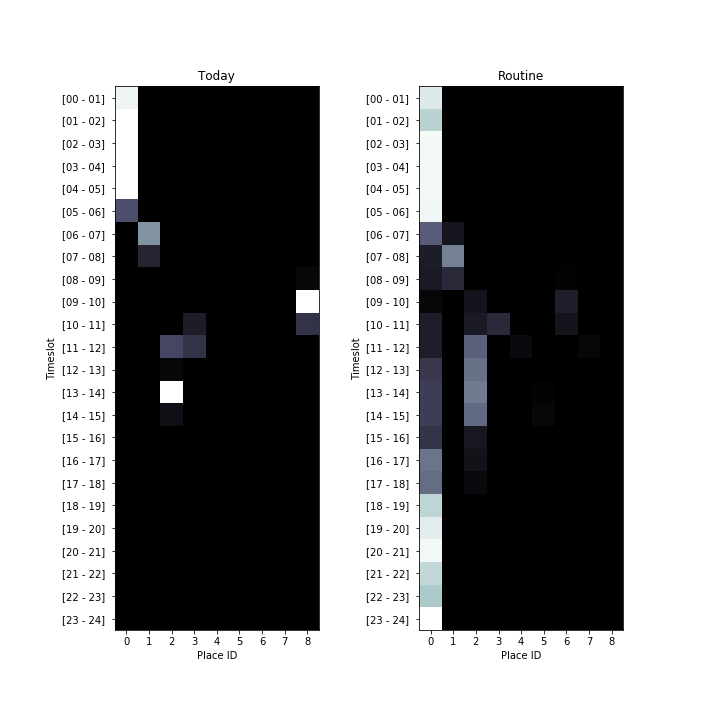
\includegraphics[width=0.5\textwidth]{images/routine.png}
    \caption{An illustration of the Hour Matrix for the a given day and the 'average day', i.e. the Routine}
    \label{fig:routine-matrix}
\end{figure}

For the overlap function we define a union operator $A \cap B$ defining the \textit{overlap} of two matrices $A$ and $B$ as 

\begin{equation}
\label{eq:overlap-function}
    A \cap B = \sum_{i=1}^{24} \sum_{j=1}^{N} \min (A_{ij}, B_{ij}) \;|\; A_{ij} \geq 0, B_{ij} \geq 0
\end{equation}

The \textit{Routine Index} for today $d_t$ given the historical dates $D$, is defined as: 

$$r(d_t, D) = \frac{\sum (\mathsf{H}(d_t) \cap \mathsf{H}^{\mu} (D) )}{\min \Big(\sum \mathsf{H}(d_t), \sum \mathsf{H}^{\mu} (D) \Big)}$$
The numerator 

$$\sum (\mathsf{H}(d_t) \cap \mathsf{H}^{\mu} (D) )$$

defines the \textit{actual overlap} as the sum of the overlapping entries between today's data and the historical data. The denominator 
$$\min \Big(\sum \mathsf{H}(d_t), \sum \mathsf{H}^{\mu} (D) \Big)$$ 

is the smallest sum of either matrix, whichever is smaller, and defines the \textit{maximum potential overlap} between the two matrices. If one matrix is very sparse then the potential overlap is very low, and vice versa. If the \textit{actual overlap} and the \textit{maximum potential overlap} are the same, it means the matrices are the same and the Routine Index will have a value of 1. 

